\documentclass[12pt]{article}
\usepackage[slovene]{babel}
\usepackage[utf8]{inputenc}
\usepackage[T2A]{fontenc}
\usepackage{amsmath}
\usepackage{amsfonts}
\usepackage{amssymb}
\usepackage[version=4]{mhchem}
\usepackage{stmaryrd}
\usepackage{graphicx}
\usepackage[export]{adjustbox}
\graphicspath{ {./images/} }
\usepackage{physics}
\usepackage{geometry}
\geometry{left=2cm,right=2cm,top=2cm,bottom=2cm}

\title{\textbf{Spektrometer}}
\author{Samo Krejan}
\date{april 2025}

\begin{document}
\maketitle

\section{Uvod}
Spektroskop je naprava za merjenje porazdelitve spektra, to je porazdelitev svetlobnega toka po frekvenci ali valovni dolžini. Glede na potrebe poznamo več različnih vrst spektroskopov, pri tej vaji pa smo uporabljali optični spektrometer na prizmo. Ta deluje, saj imajo različne valovne dolžine različne lomne količnike, tako da ko se svetloba lomi, pod različnimi koti vidimo različne komponente spektra. Ako bi na prizmo posvetili z zvezno svetlobo, bi na drugi strani videli mavrico, ča pa posvetimo s svetilom z diskretnim spektrom, pa vidimo posamezne komponente.

Ker kot detektor svetlobe / valovanja uporabljamo kar oko, se moramo zavedati njegovih pomankljivosti. Z očesom namreč vidimo zgolj zelo omejen del spektra in še preko spektra vidimo različno svetlobo različno dobro. Zeleno vidimo najbolje, tudi 100 krat bolje kot vijolično in rdečo, ki sta obe na robu vidnega spektra. To dejstvo dobro ponazarja slika \ref{oko}:

\begin{figure}[ht]
\begin{center}
    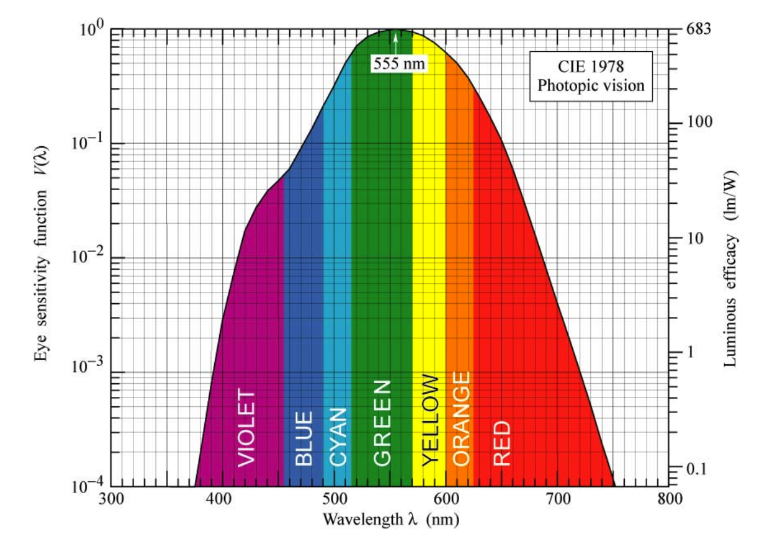
\includegraphics[width=10cm]{oko.png}
    \caption{Občutljivost očesa}
    \label{oko}
\end{center}
\end{figure}

Kot omenjeno optični spektrometer na prizmo temelji na pojavu disperzije, to je efekt, zaradi katerega imajo različne valovne dolžine različne lomne količnike. Odvisnost lomnega količnika od valovne dolžine zelo dobro opiše Seillmeierjeva formula \ref{Seill}:

\begin{equation}
    n(\lambda)^2 = 1 + \frac{A\lambda ^2}{\lambda ^2-\lambda_0^2}
    \label{Seill}
\end{equation}

\section{Potrebščine}
\begin{itemize}
    \item Optični spektrometer; prizma iz kremenastega stekla,
    \item nosilec za spektralne cevi (ampule) z visokonapetostnim izvirom, ampule s plini He, Ne, Hg, H2,
    \item varčna žarnica, LED diode, wolframova žarnica, cevka z NO2.
\end{itemize}

\section{Naloga}

\begin{enumerate}
    \item Umerite kotno skalo s spektralnimi črtami Hg in H2,
    \item izmerite valovne dolžine spektralnih črtv spektru varčne žarnice. Primerjajte spekter s tistim, izmerjenim v Hg,
    \item izmerite centralno valovno dolžino in ocenite spektralno širino svetlečih diod različnih barv,
    \item opazujte zvezni spekter wolframove svetilke in ocenite valovno dolžino najsvetlejšega dela spektra, ter določite intervale, ki jih pokrivajo določene barve,
    \item opazujte absorbcijski spekter NO2,
    \item izmerite valovne dolžine črt v spektru Ne in He.
\end{enumerate}


\section{Rezultati in analiza}
Najprej smo izmerili tri najbolj intenzivne (in najbolj zanesljive) črte iz spektra Hg in H2. Te črte smo uporabili, za umeritveno krivuljo, ki povezuje kot opazovanja z valovno dolžino. Krivulja ima obliko \ref{umeritev}:

\begin{equation}
    \phi = c_1 + c_2\lambda + c_3\sqrt{\lambda}
    \label{umeritev}
\end{equation}

To funkcijo smo "pofittali" na naše podatke in tako dobili naslednje vrednosti za parametre $c_i$:

\begin{equation*}
    mjav mjav woof woof
\end{equation*}


\end{document}